\title{Comment on ``Causal inference using invariant prediction''}
\author{Trevor Hastie, Robert Tibshirani, Qingyuan Zhao, Charles Zheng}
\date{\today}

\documentclass{article}

% packages with special commands
\usepackage{amssymb, amsmath}
\usepackage{epsfig}
\usepackage{array}
\usepackage{ifthen}
\usepackage{color}
\usepackage{fancyhdr}
\usepackage{graphicx}
\usepackage{mathtools}
\usepackage{csquotes}
\usepackage[authoryear]{natbib}
\definecolor{grey}{rgb}{0.5,0.5,0.5}

\begin{document}
\maketitle

\newcommand{\tr}{\text{tr}}
\newcommand{\E}{\textbf{E}}
\newcommand{\diag}{\text{diag}}
\newcommand{\argmax}{\text{argmax}}
\newcommand{\Cov}{\text{Cov}}
\newcommand{\Var}{\text{Var}}
\newcommand{\argmin}{\text{argmin}}
\newcommand{\Vol}{\text{Vol}}
\newcommand{\comm}[1]{}

We congratulate the authors on this thought-provoking
paper. Statistical inference of causality has been thoroughly studied
in randomized experiments or observational studies, but is seldom
considered when data from both \emph{observational}
and \emph{interventional} settings are available. Peters et
al.\ made an important contribution by tackling this problem with
their notion of invariant causal prediction (ICP).

At first look, the ICP is just a corollary of structural
equation models, but we think its value might be much more
substantial. Given a response variable, ICP can discover its invariant
prediction sets, in some sense its
``causes''. \citet{holland1986statistics}, \citet{dawid2000causal},
\citet{pearl2000causality}, among many others, suggest that we should
distinguish between the problem of ``effects of causes'' and ``causes
of effects''. As argued by \citet{robins2000causal} and
\citet{pearl2000causality}, a counterfactual language is usually
required to study the latter problem. Does ICP enable us to study
``causes of effects'' without counterfactuals? Although ICP is
motivated by structural models which naturally encodes
counterfactuals, ICP seems not to involve any counterfactual term. We
hope the authors can answer this question in the rejoinder.

We think the concept of invariant prediction is quite
general and goes beyond a specific modeling assumption. Unfortunately,
most of this paper is devoted to the linear model with noise and
generalizations of ICP to more flexible models (GLMs,
nonparametric models, non-additive models) would be extremely useful
in practice.

We evaluated ICP on a protein signaling network dataset of
\citet{sachs2005causal} using the software provided by the authors.
\citet{sachs2005causal} collected a
combination of observational and interventional data to infer the
causal structure of a network consisting of 11 proteins.  Using their
own method, \citet{sachs2005causal} reportedly recovered 15 of the
known directed arcs (colored black in Figure \ref{fig:sachs}) and
discovered two new putative links (not shown), and missed 3 of the
interactions which were known in the literature (dashed lines). We
tried to use ICP to recover part of the graph structure: ICP
discovered one arrow correctly and two incorrect arrows. No other
discoveries were reported.

\begin{figure}[t]
\centering
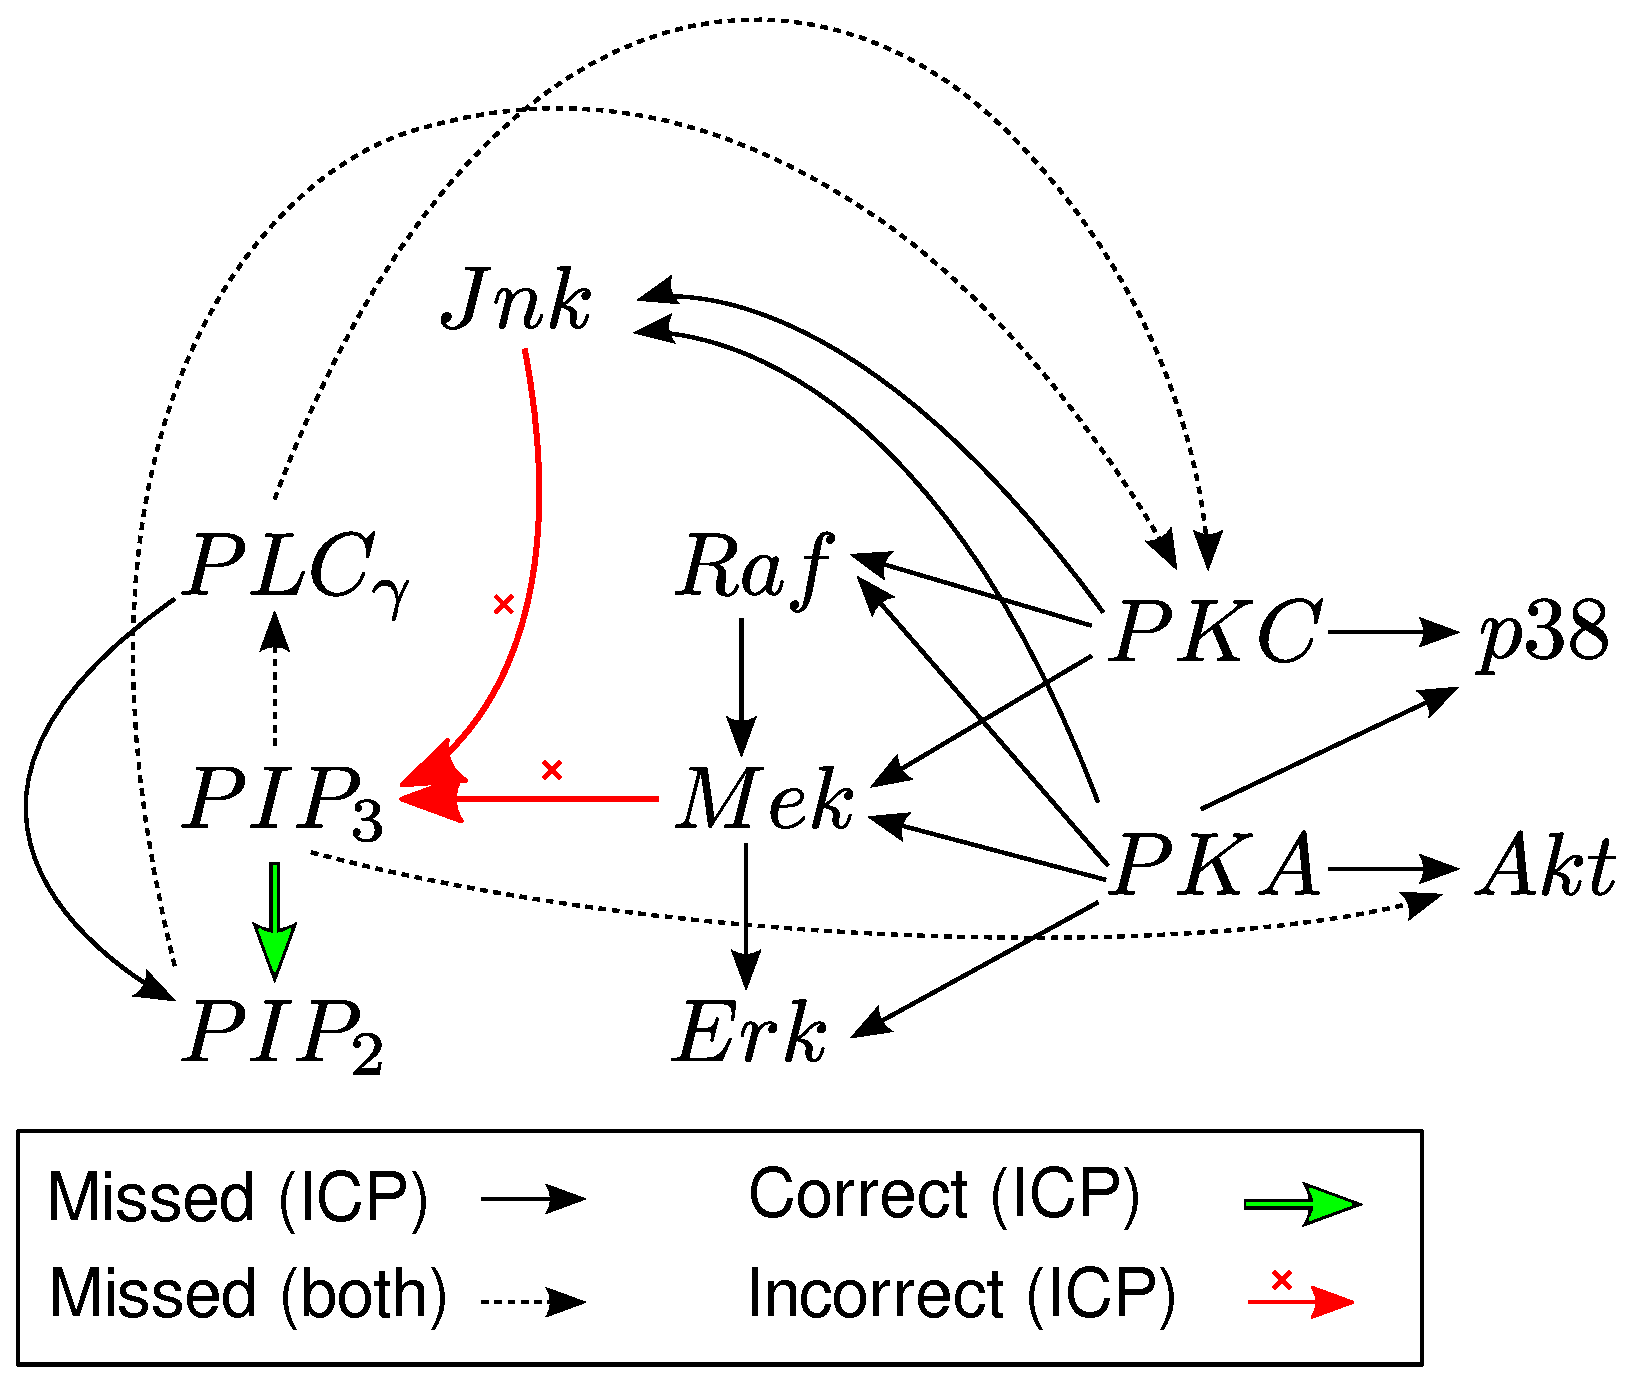
\includegraphics[scale = 0.3]{drawing2legend.eps}
\caption{Application of ICP procedure to recover protein signaling network,
taking in turn each of the 11 variables as the response of interest
and selecting the subset of environments in which the response was not
perturbed.  The invariant set for each variable can be identified as
the parents of that variable in the graph.  For 9 of the 11 proteins,
ICP rejected the model and reported no discoveries.  For the protein
PIP2, ICP correctly identified one parent, PIP3.  For the protein
PIP3, ICP reported Mek and Jnk as part of the invariant set, but these
do not match any interactions known in the literature.}
\label{fig:sachs}
\end{figure}

The overly-restrictive linear model could be the reason for the poor
performance of ICP on this dataset. The authors take this as a
robustness property, but it also means ICP is very sensitive to
modeling assumptions. A small departure from the linear
model can result in no causal discovery. We did not find in the paper a
summary of the robustness of ICP, so we tried to outline in
Table \ref{tab:icp} the behavior of linear ICP when some of its
assumptions are not met. We would welcome the authors' comments on
this summary.


\begin{table}[h]
\centering
  \begin{tabular}{c|c|c|}
    \hline
    &\textbf{Issues} & \textbf{ICP's behavior} \\
    \hline
    a) & Intervene on $Y$ (or a missing cause) &
    $\underset{\emptyset}{\bigcap}$ \\
    \hline
    b) & Non-linear, non-additive, and/or heteroscedastic &
    $\underset{\emptyset}{\bigcap}$ \\
    \hline
    c) & Not enough interventions &
    \textcolor{red}{False causal positives} \\
    \hline
    d) & Small sample size &
    $\emptyset$ \\
    \hline
    e) & Left out a confounder & $\underset{\emptyset}{\bigcap}$ \\
    \hline
    f) & Left out an unconfounding predictor & okay  \\
    \hline
    g) & Misspecified noise model$^2$ & \textcolor{red}{False positives}\\\hline
  \end{tabular}
\caption{Robustness properties of the ICP procedure.  Under certain types
  of model misspecification, ICP will return a ``model reject'',
  denoted by $\cap_{\emptyset}$ (i.e.\ all subsets including the empty
  set are not invariant), rather than produce false positives.
(a) when interventions are performed on $Y$, no predictor set can be invariant;
(b) when the homoscedastic linear model is misspecified, the prediction rule
will vary depending on the range of the predictors; (c) without enough interventions,
the set of causal parents is unidentifiable, and non-causal invariant sets exist;
(d) when the sample size is small, the hypothesis test for invariance has insufficient power to reject the invariance null,
hence many sets are accepted as invariant;
(e) if a confounder is left out, this is equivalent to intervening on $Y$;
(f) when an uncounfounding predictor is left out, its effect is equivalent to i.i.d. noise;
(g) under a misspecified noise model, the hypothesis test may not be sensitive to differences in the noise distribution,
leading to low power.
}
\label{tab:icp}
\end{table}


\bibliographystyle{plainnat}
\bibliography{ref}


\end{document}
